\label{sec:field}

\section{Geometry}

The steady reduced order model (ROM) was used to explore a broad set of
system configurations and to optimize kinetic energy flux. The resulting
configuration represents a significant change from that used in the
August 2015 Field test. Horizontal and vertical views of this
configuration are shown in Figures \ref{a-b}, below. A brief summary of
the differences is given below: 

\begin{itemize}
\item The bottom tier vanes are significantly taller than in the field.
\item An impermeable cylinder was introduced along the arc $\{\pi < \theta
      < 0 \}$, e.g. the bottom two quadrants in the images below, replacing the
vanes in those quadrants. 
\item The cone is taller providing a greater contraction.
\item The bottom tier vanes are no longer symmetric: the downwind side is
taller because the downwind boundary layer is thicker and has a lower
peak turning angle to reduce blockage.
\item The upper tier vanes were configured to align with the freestream
velocity, to provide a larger wind-driven flux into the facility.
\item Horizontal partitions were added to the top of the upper vanes, to
prevent flow in the vanes from rising up and out of the vanes. 
\end{itemize}

 \begin{figure}[!htb]
  \begin{center}
   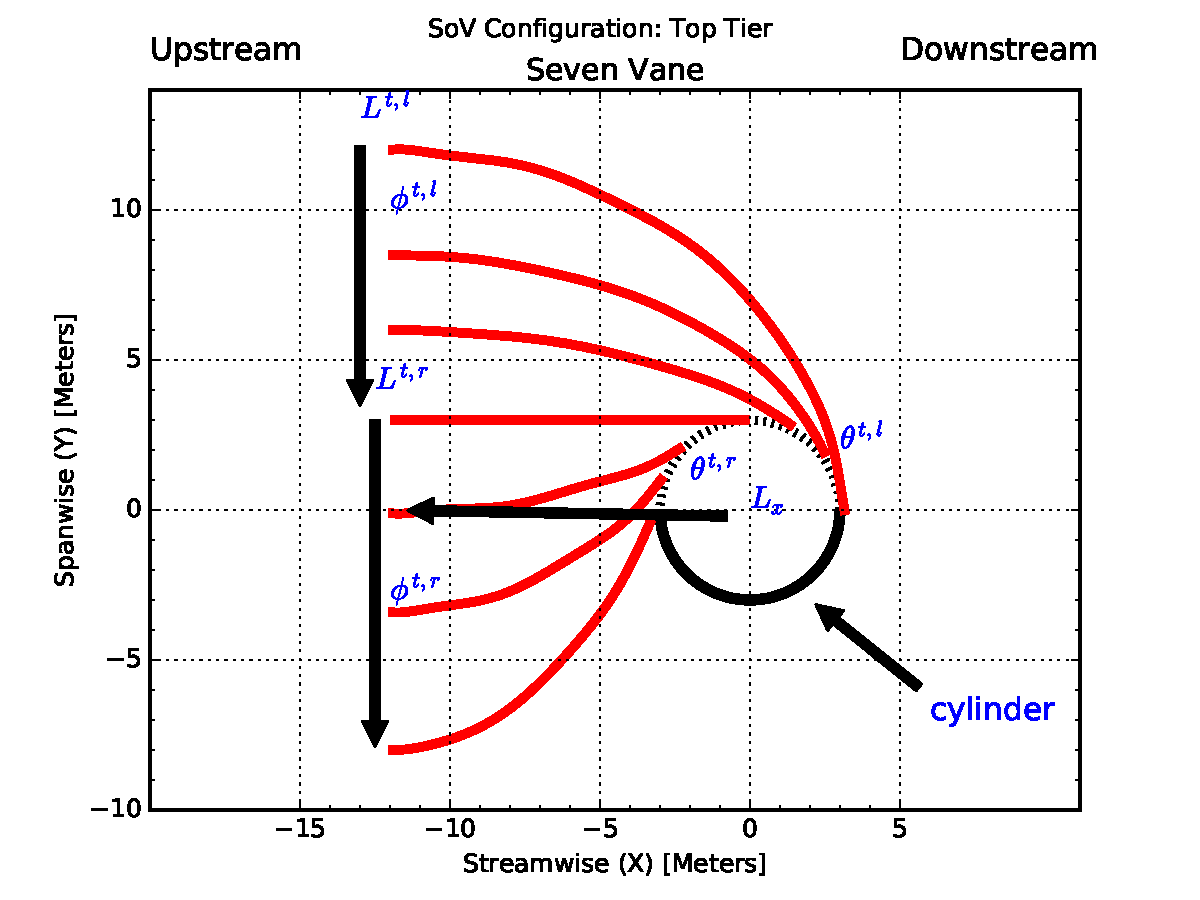
\includegraphics[width = 13 cm]{figs/interp_entire_top.pdf}
   \caption{A top view of the top vane design. The red lines are the
     vanes, which are spaced so that the mass flux between vanes is
     approximately equal. The blue symbols are the parameters that
     specify the design. Notice the highly asymmetric configuration,
     with the front (left) opening of the vanes aligned directly with
     the incoming wind.}
   \label{fig:top_design}
  \end{center}
 \end{figure}

\begin{table}[]
\centering
\begin{tabular}{lll}
Name                        & Value & Meaning                    \\
 \hline
$r^{\text{cyl}}$            &  3.0 meters & radius of rigid cylinder \\
$r^t_{\text{min}}$          &  3.0 meters & smallest radius of top tier
	 vanes, relative to ground \\
$L_x$                       &  12 meters  & Distance upstream
	 of vanes relative to center\\
$\phi^{t,l}$ &  $0^{\circ}$   & Outer angle for the top tier, left side vanes \\
$\phi^{t,r}$   &  $0^{\circ}$   & Outer angle for the top tier right side \\
$\theta^{t,l}$ &   $30^{\circ} +\frac{\alpha}{3}$  & Inner angle for the top tier left side vanes\\
$\theta^{t,r}$   &   $75^{\circ} +\frac{\alpha}{6}$   & Inner angle for the top tier right side \\
$L^{t,r}$                   &  12 meters  & width of vane in front of cylinder \\
$L^{t,l}$                   &  10 meters  & width of vane to the side of cylinder \\
\end{tabular}
\end{table}

\begin{itemize}
 \item $\phi$  angle relative to streamwise direction ($\hat i$)
 \item $\theta$ angle relative to radial direction ($\hat r$)
 \item $\alpha$ is angle from origin to inner terminus of vane
 \item Superscript $t$ denotes top, $l$ is left, $r$ right (when viewed
       from front)
 \item Forcing function has a discontinuity at $\alpha=90^{\circ}$
\end{itemize}

 \begin{figure}[!htb]
  \begin{center}
   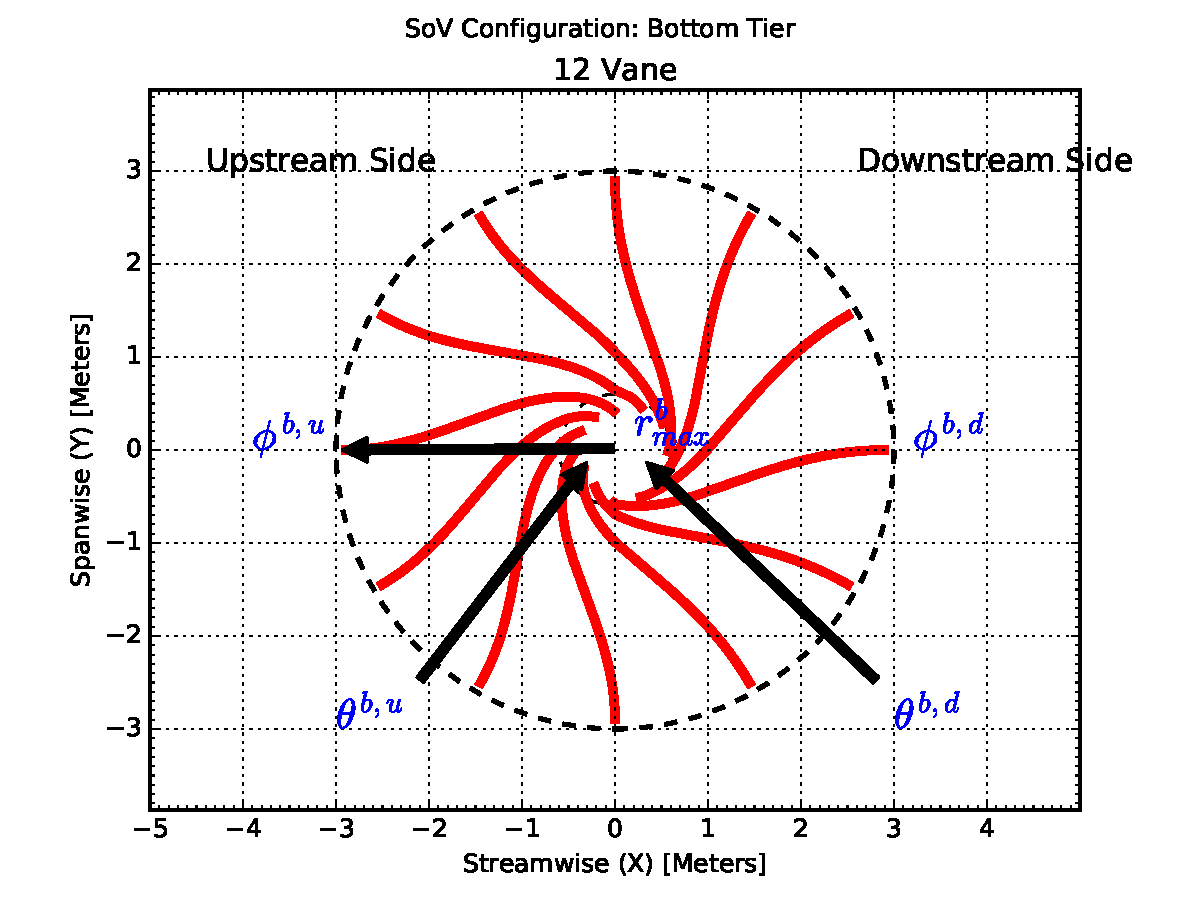
\includegraphics[width = 13 cm]{figs/interp_entire_bottom.pdf}
   \caption{A top view of the bottom tier design. These vanes (in red)
   are also asymmetric, with lower final curvature angles and a taller
   height for the back (downstream) vanes versus the front. This is due
   to the thicker boundary layer of the flow entering the device from
   the right (downstream relative to the wind). These vanes are design
   to turn the incoming flow so that it is nearly azimuthal near the
   center of the apparatus, increasing rotation and lowering the
   pressure in the center.}
   \label{fig:bottom_design}
  \end{center}
 \end{figure}

\begin{table}[]
\centering
\begin{tabular}{lll}
Name                        & Value & Meaning                    \\
 \hline
$r^b_{\text{min}}$          &  0.6 meters & Smallest radius of bottom tier vanes \\
$r^b_{\text{max}}$          &  6.0 meters & Largest radius of bottom tier vanes \\
$\theta^{b,d}$ &  $60^{\circ}$   & Inner angle for the bottom tier, downstream vanes \\
$\theta^{b,u}$ &  $80^{\circ}$   & Inner angle for the bottom tier, upstream vanes \\
$\phi^{b,d}$ &   0   & Outer angle for the bottom  tier, downstream vanes \\
$\phi^{b,u}$ &   0   & Outer angle for the bottom tier, upstream vanes \\
\end{tabular}
\end{table}

\begin{itemize}
 \item Superscript $b$ denotes bottom tier, $d$ is downstream, $u$ upstream vanes
 \item $\phi$,$\theta$ angles relative to radial ($\hat r$)
\end{itemize}


\begin{figure}[!htb]
  \begin{center}
   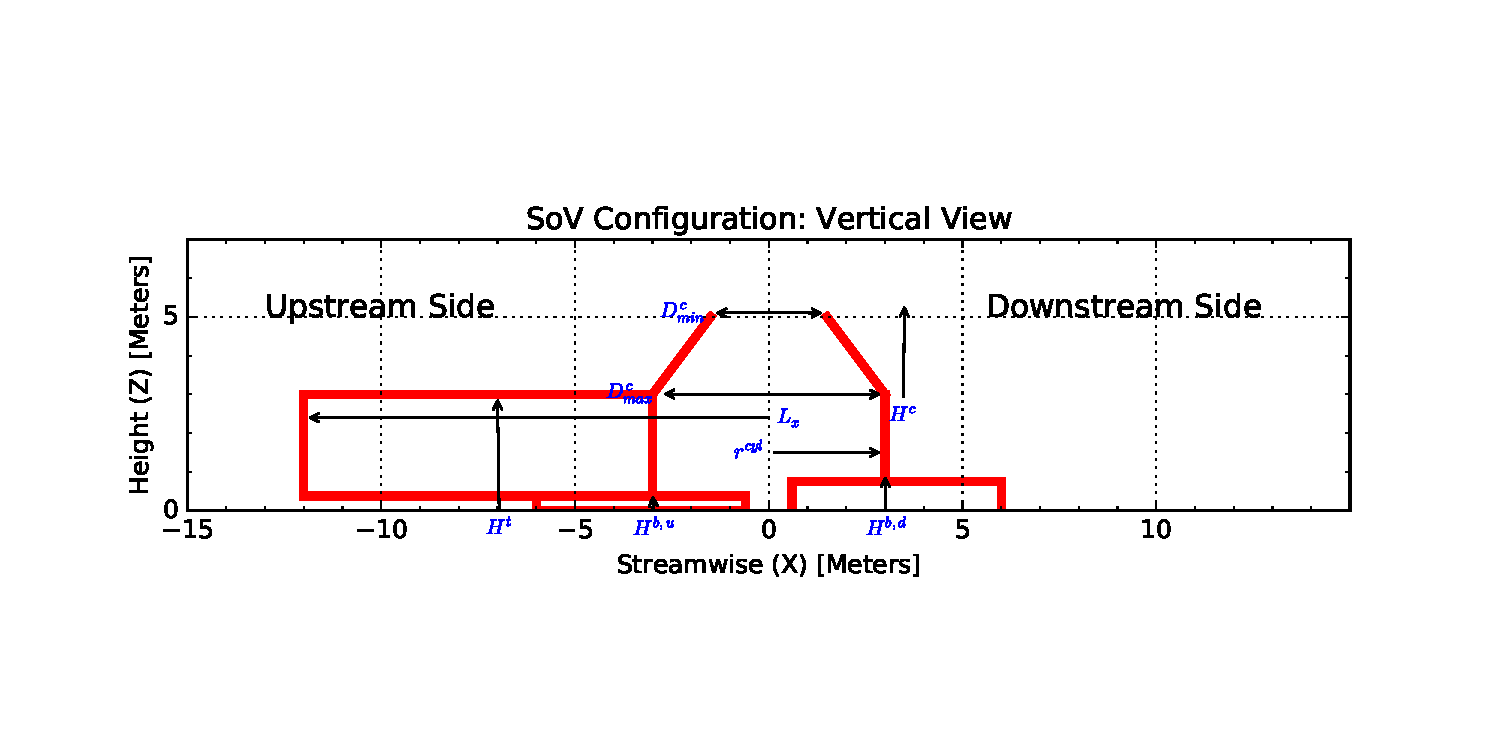
\includegraphics[width = 15 cm]{figs/vertical_design.pdf}
   \caption{A side view of the summer 2016 two tier vane design. The
     vanes are drawn in red. The difference in heights between lower
     tier vanes in front and back vanes is clearly visible. The turbine
     is placed at the top of the cone.}
   \label{fig:vertical_design}
  \end{center}
 \end{figure}

\begin{table}[]
\centering
\begin{tabular}{lll}
Name                        & Value & Meaning                    \\
 \hline
$r^{\text{cyl}}$            &  3.0 meters  & radius of rigid cylinder \\
$L_x$                       &  12 meters  & Furthest distance upstream of top	 tier vanes \\
 $H^t    $                  &   3 meters  & Height of top tier vanes \\
 $H^{b,u}$                  & 0.375 meters & Height of bottom tier, upstream vanes \\
 $H^{b,d}$                  &   .75 meters& Height of bottom tier, downstream vanes \\
 $H^{c}$                    &   2 meters  & Cone Height \\
 $D^c_{\text{min}}    $     &   3 meters  & Minimum cone diameter \\
 $D^c_{\text{max}}    $     &   6 meters  & Diameter of cone at top of vanes\\
\end{tabular}
\end{table}


The top tier design is now highly asymmetric, with a
large opening facing the incoming wind to capture incoming free stream
kinetic energy over a large area. The incoming flow enters the central
cylindrical area, where it spins and is driven out the top through the
cone. 

To enable these more general vane geometries for the top tier, it was
necessary to formulate a more general parameterization of the
vanes.\todo{why did we need to do this?} 

Previously, the vanes had a linear curvature function and were
axisymmetric. The new concept required the vanes to hold an azimuthal
dependence so that they are aligned with the streamwise velocity upsteam 
of the device, and then curve inward to spin the flow at the center of
the device. A linear vane curvature was first attempted, but this was
found to have too few degrees of freedom to provide adjustments to the
vane curvature. Next, vanes that had an elliptic curvature were decided
upon. The intent here is to have a quarter of an ellipse, where the arc
of the ellipse starts at the x-intercept (thus ensuring the vane is
aligned with the freestream velocity) and then curves in towards the
center of the device, terminating at a high angle nearly azimuthal. To
accomplish this, the normal vector of the ellipse must be known. 

This required use of implicit differentiation for the functional,

\begin{eqnarray}
 f(x,y)  =& \frac{(x-h)^2}{a^2} + \frac{(y-k)^2}{b^2} = 1, \\
 \nabla f(x,y) =& \frac{2 (x-h)}{a^2} + \frac{2 (y-k)}{b^2}\frac{dy}{dx} = 0, \\
 \frac{dy}{dx} =& -\frac{(x-h)}{(y-k)}\frac{b^2}{a^2}. 
\end{eqnarray}
Where h and k are the elliptic intercepts and a and b are the
eccentricity of the ellipse along each axis. The tangent vector along
the ellipse is then,  
\begin{eqnarray}
 %{\bf \hat t} = {\bf e_x} + \frac{dy}{dx}{\bf e_y}, \\
 {\bf t} =& {\bf e_x} + \frac{dy}{dx}{\bf e_y}, \\
 {\bf t} =& \underbrace{\frac{(y-k)}{b^2}}_{a_y} {\bf e_x} +
  \underbrace{\frac{(x-h)}{a^2}}_{a_x}{\bf e_y} \\
 {\bf t} =& {a_y} {\bf e_x} + {a_x}{\bf e_y}
\end{eqnarray}


The virtual vane function is now specified by a 2D N\textsuperscript{th}
order polynomial fitted to the boundary constraints for the vane angle
within the region of the vanes. This has the form, 

\begin{equation}
 P(x,y) = \sum_{i=0}^N  \sum_{j=0}^N a_{i,j} x^i y^j
\end{equation}

where $a_{i,j}$ are coefficients of the polynomial which are selected by
minimizing the residual between the specified vane values and the
polynomial evaluated at that point. In other words, we find the
least-squares solution to a linear matrix equation, which is
under-determined. The solution to the equation $A x = b$ is found by
computing a vector $x$ that minimizes the Euclidean 2-norm $|| b - A x
||^2$. The polynomials were computed in separate python routines and
resulted in a generated input file. This was then used as part of the
input for the field runs (see Appendix~\ref{sec:archiving} for more
details on the input file environment). 

%
% http://docs.scipy.org/doc/numpy-1.10.0/reference/generated/numpy.linalg.lstsq.html
%

e.g.\todo{show 7th order}

 \begin{figure}[!htb]
  \begin{center}
   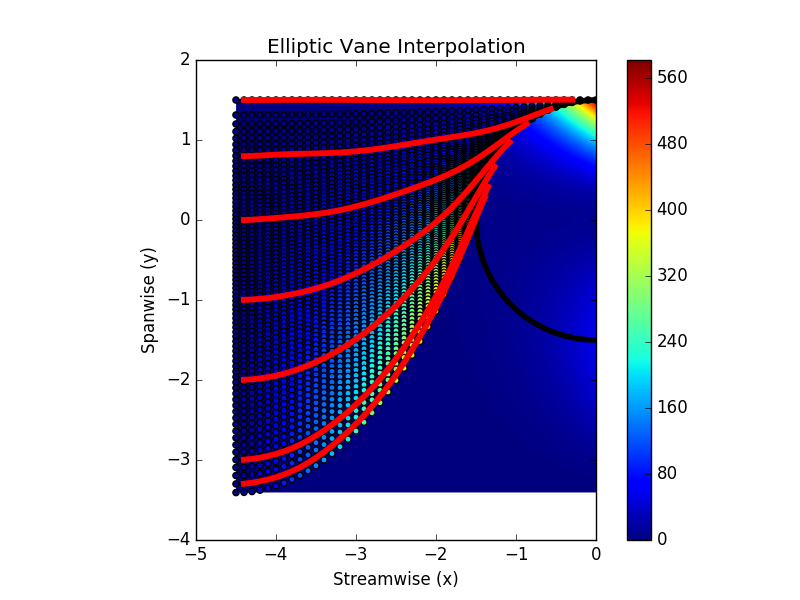
\includegraphics[width = 15 cm]{figs/bottom_interp}
   \caption{Top view of the interpolation function for the ``right
   side'' of the vanes on the top tier. The red lines are the data sets
   that provides the input data used to calibrate the two dimensional
   polynomial field. The black line is the inner radius of the SoV.}
   \label{fig:bottom_interp}
  \end{center}
 \end{figure}

The polynomial order was selected to be 7\textsuperscript{th} because it
provided a good balance between accuracy and a desire to maintain as low
an order as possible. Furthermore, the vanes interpolation was split
into two components, for the ``left'' and ``right'' (from the perspective of a
person standing upwind of the SoV and looking at it) of the vanes in the
top tier. The ``right'' interpolated field is shown in
Figure~\ref{fig:bottom_interp}.\todo{update python plots} 

%
% /h2/nick/src/code/python/poly_vanes
%

The optimized configuration for this case results in 3.05 kW of kinetic
energy flux through the top of the vanes, which is 417\% more kinetic
energy flux than was produced in the August 2015 Field test.

An optimal set of design parameters were determined and provided to the
experimental group, for detailed mechanical design and
fabrication.\todo{add some pretty CAD drawings}

Provided by Mr. John Culp at Georgia Tech. 


\section{Field Prediction}
\label{subsec:field_predict}

also show fields and images

\section{Sources of Error}

%\section{Effect if the Cone}
%
%behaves like wind tunnel contraction

Scenario Uncertainty

Shading

Actuator disk under-estimates drag

no model for drag on vanes (was reported by team)

transient before spin up

\section{Turbine Design}

  \begin{figure}[!htb]
   \begin{center}
    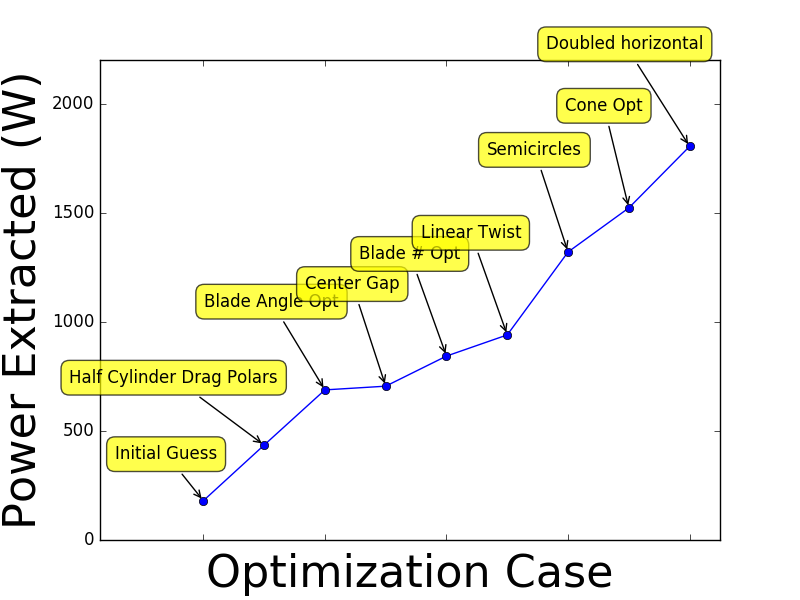
\includegraphics[width = 10 cm]{figs/turbine_opt}
    \caption{Turbine optimization}
    \label{fig:ut_turbine}
   \end{center}
  \end{figure}

In addition to the final vane design, a turbine design developed in
collaboration with Duane McCormick at UTRC. This design was arrived at
by coupling a ``frozen flow'' optimization routine from UTRC with a Blade
Element Momentum (BEM) rotor model integrated into UT's CFD model as an
actuator disk. The rotor/inflow coupling directly modeled enabling
accurate rotor inflow predictions. In this way, the UTRC code would
iterate through design parameters using the coupled CFD code as a higher
fidelity confirmation. The UTRC frozen flow optimization was largely
consistent with the fully coupled CFD prediction (see Figure \ref{},
below). This has resulted in two final rotor designs, with and without
twist. This was because the experimental team was not certain that a
twisted design would be feasible. Regardless, the twisted rotor
out-performed the zero-twist rotor. The peak power extracted is
predicted to be 1.4 kW for the rotor with twist, and slightly more than
1 kW for a rotor with no twist. 

  \begin{figure}[!htb]
   \begin{center}
    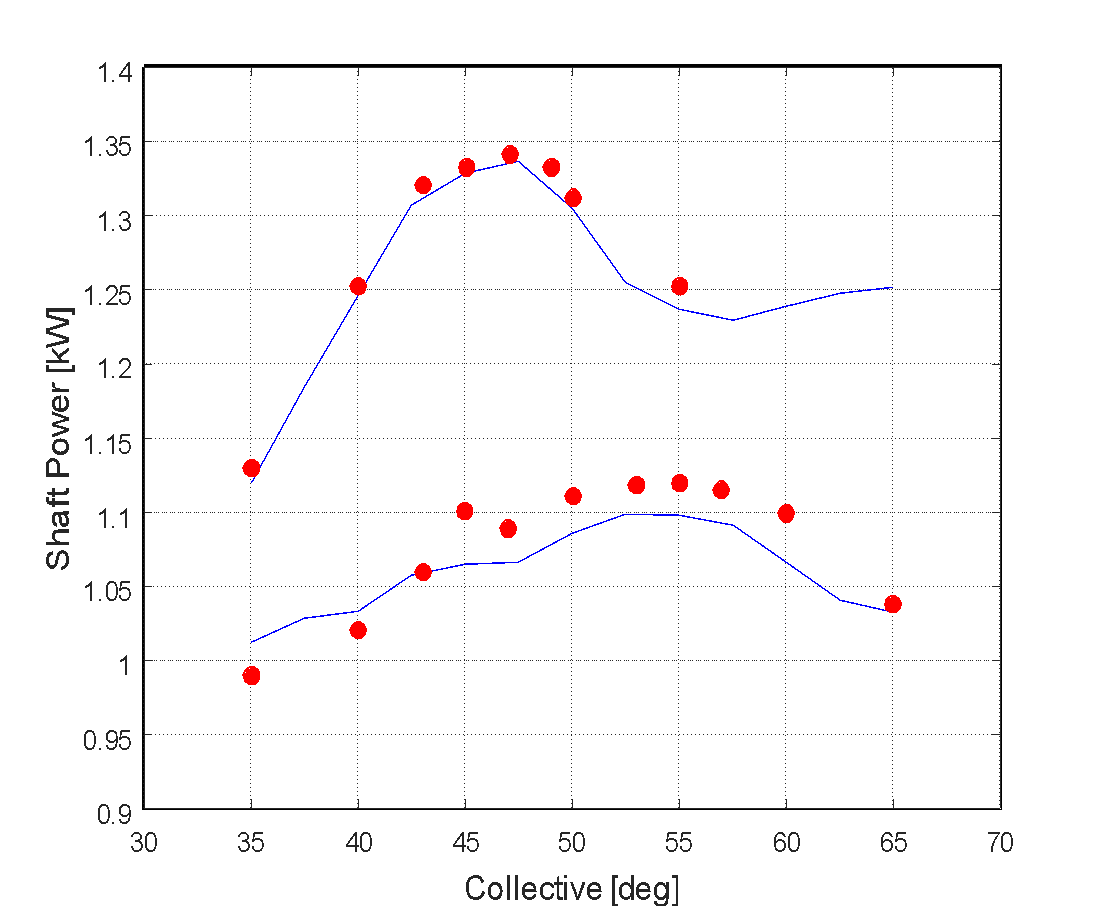
\includegraphics[width = 10 cm]{figs/utrc_plot}
    \caption{The power extracted by the rotor predicted by the CFD (red
    circles) and ``frozen flow'' (blue line) for a range of rotor
    collective angles. The higher lines are for blades with twist, and
    the lower are for constant blade angle runs, which was always
    inferior in terms of power extracted.}
    \label{fig:UTRC_turbine}
   \end{center}
  \end{figure}


In general, the frozen flow and fully coupled CFD agree. However this is
only for rotor loadings close to those in the coupled CFD. The errors
tend to be in frozen flow predictions with parameters far from the
coupled CFD. In some cases, the limitations of the frozen flow
optimization were significant. For instance, several attempts
to extract more power at large RPMs would cause a breakdown of SoV
flow in the coupled CFD model, which resulted in the flow power dropping
by more than an order of magnitude.\todo{add turbine flow pictures}

Add turbine table\todo{add table with turbine}

  \begin{figure}
   \centering
   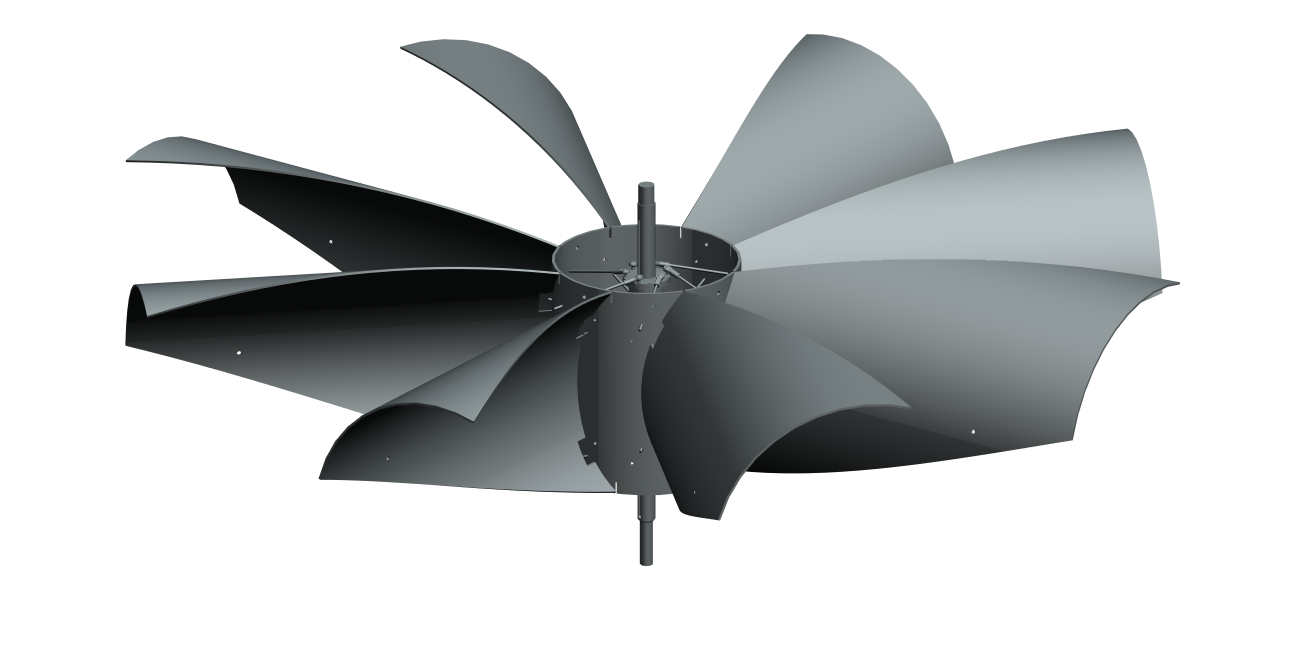
\includegraphics[width =0.45\textwidth]{figs/rotor_assem_oblique_1}
   \hfill
   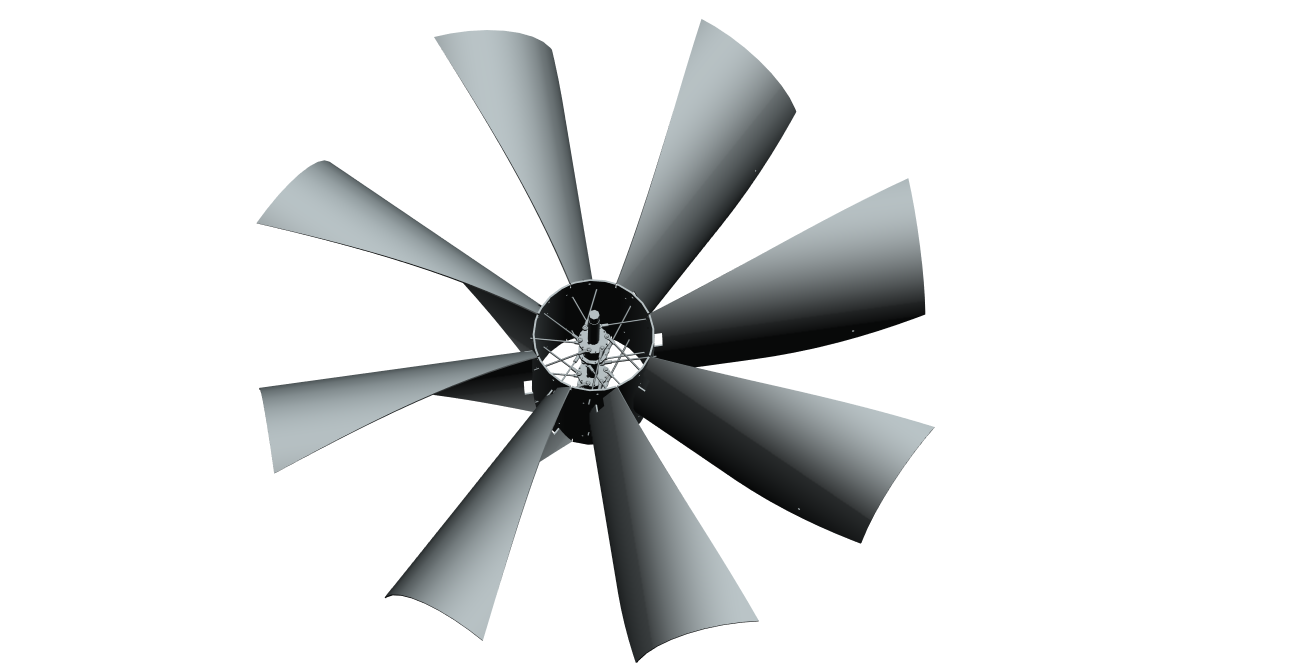
\includegraphics[width =0.45\textwidth]{figs/rotor_assem_oblique_2}
   \\
   \vspace{1em}
   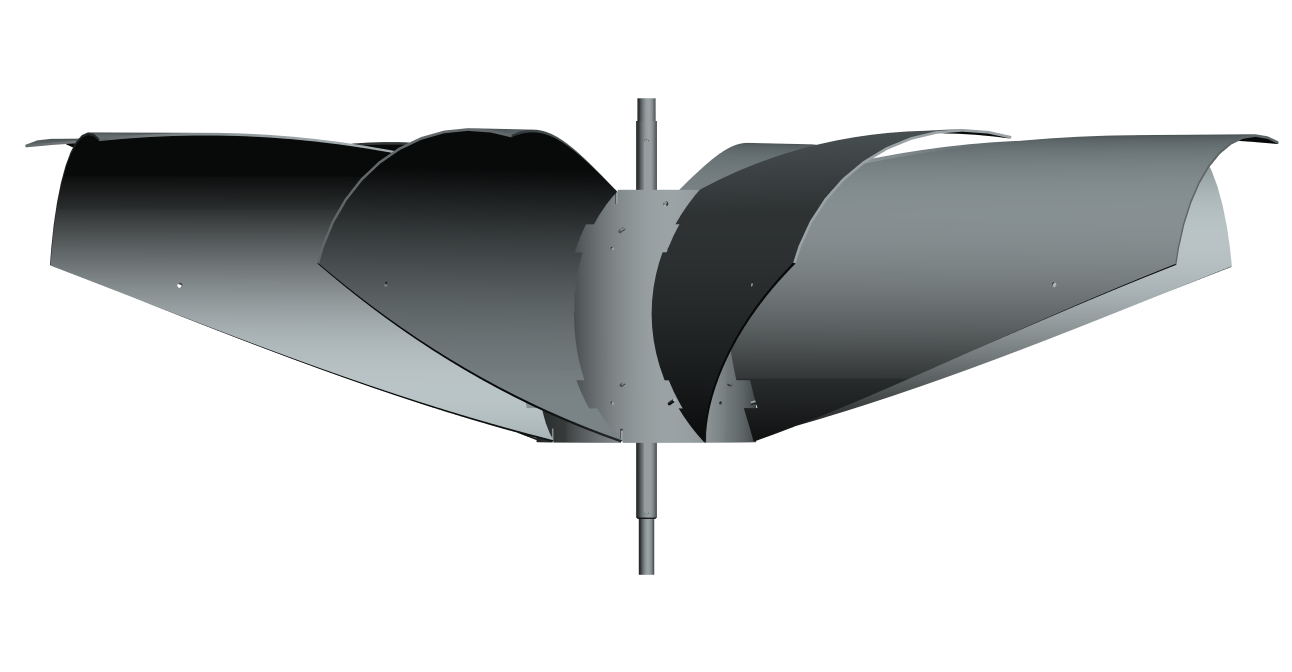
\includegraphics[width =0.45\textwidth]{figs/rotor_assem_side_render}
   \hfill
   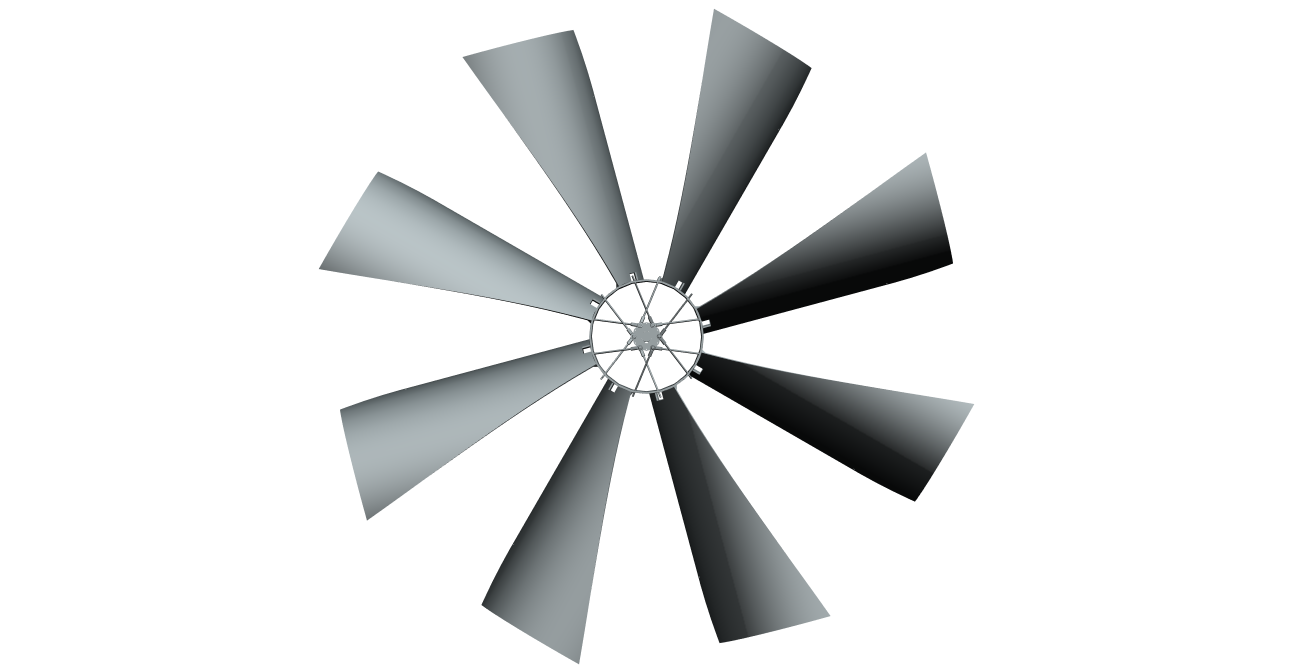
\includegraphics[width =0.45\textwidth]{figs/rotor_assem_top}
   \\   
   \caption{CAD design images of the turbine} 
   \label{fig:cad_turbine}
  \end{figure}


  \begin{figure}
   \centering
   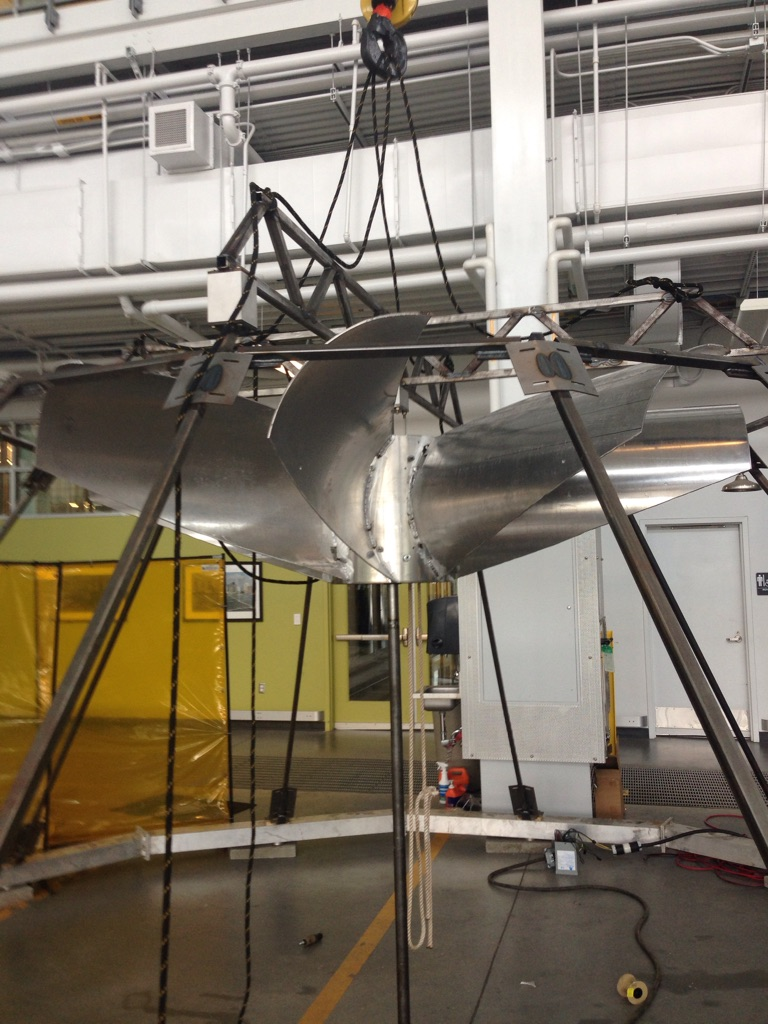
\includegraphics[width =0.45\textwidth]{figs/turbine_built}
   \caption{The fabricated turbine.} 
   \label{fig:turbine_built}
  \end{figure}

Shortcomings -- \todo{finish me}

Designed for axisymmetric flow. No wake correction as depicted in
Section\ref{subsec:wake_loss_model}.    

\section{Determining the Optimal Drag Polars}

All of the results in section \ref{subsec:field_predict} were generated
using 90 degree semicircle blade geometries, as shown in Figure
\ref{fig:90_drag}. A natural question then is whether more power might
be extracted with a different rotor geometry. While several comparisons
have been performed with different choices of drag polars (flat plate,
180 degree semicircles, etc. ) this was not an exhaustive survey. 

Practical utility-scale wind turbines achieve at peak 75\% to 80\% of
the Betz limit\cite{?}. While this provides an estimate, the Betz-limit
is likely not accurate for this case. Any analysis of the power that can
be extracted is complicated by the presence of considerable vertical and
azimuthal flow in the vortex, and so the design considerations are
different from those for a classical wind turbine.

To address the possible possibility of further turbine blade
improvements, this section details a more generic set of drag
polars. These generalized drag polars permit exploration of a broader
design space. The optimization of this model can be fully coupled to the
flow, and so does not violate any Betz-like considerations that might
similarly arise in an analysis of frozen flow fields.
The drag polars are selected to be generic functions and are optimized to
maximize the power extracted by the rotor. While the resulting drag
polars might not be physically  realizable, they represent a ``best
case'' upper bound indicating the peak power that might be extracted
with further rotor design iterations. This ``limiting case'' is useful
for evaluating the system feasibility from a technological standpoint,
by providing the peak power that could be extracted for a given vane
geometry. 

The power extracted by the turbine is, 
\begin{equation}
 P = \Omega Q
\end{equation}
where the torque, Q, is, 
\begin{equation}
 Q = A_R \int_0^{2\pi} \int_{r_{\text{min}}}^{r_{\text{max}}} F''_{\tau}\, r\, dr d\theta.
\end{equation}
Here, $A_R$ is the relative area coefficient which is, 
\begin{equation}
A_R = \frac{c B (r_{\text{max}}-r_{\text{min}})}{\pi(r_{\text{max}}^2-r_{\text{min}}^2)}
\end{equation}
where B is the number of blades, $r_{\text{max}}$ and $r_{\text{min}}$
are the turbine radii, and $F''_{\tau}$ is the force per unit
area on the turbine, which is, 
\begin{equation}
 F''_{\tau} = \frac{F_{\tau}}{cl}= \frac{1}{2}\rho U_R^2 \, C_{\tau}.
\end{equation}
with $U_R$ the magnitude of relative velocity and $c$ is the blade chord
length, which is assumed to be constant (not a function of the radius,
for instance). Finally, $C_{\tau}$ is the tangential force coefficient,
which depends on the local lift and drap coefficients, and the
flow angle, $\phi$, 
\begin{equation}
 C_{\tau} = C_L \,\text{sin}(\phi) + C_D \,\text{cos}(\phi)
\end{equation}
Combining the equations above results in an expression for the power
that explicitly depends on the lift and drag coefficients, 
\begin{equation*}
 P = \frac{\Omega \rho c B (r_{\text{max}}-r_{\text{min}})}{2 \pi(r_{\text{max}}^2-r_{\text{min}}^2)}
\int_0^{2\pi}
\int_{r_{\text{min}}}^{r_{\text{max}}} U_R(r,\theta,\Omega)^2 \left(C_L
						     \,\text{sin}(\phi)
						     + C_D
						     \,\text{cos}(\phi)
						    \right) r\,dr d\theta. 
\end{equation*}
We lump the constant terms together, $E_{\tau} = \frac{\Omega \rho c B (r_{\text{max}}-r_{\text{min}})}{2 \pi(r_{\text{max}}^2-r_{\text{min}}^2)}$ and separate this equation, 
\begin{align}
 P_L = E_\tau
 \int_0^{2\pi}
  \int_{r_{\text{min}}}^{r_{\text{max}}} U_R(r,\theta,\Omega)^2 \, C_L(\phi,r)
 \,\text{sin}(\phi)\, r\,dr d\theta,  \label{lift} \\
 P_D = E_\tau
 \int_0^{2\pi}
  \int_{r_{\text{min}}}^{r_{\text{max}}} U_R(r,\theta,\Omega)^2 \, C_D(\phi,r) \,\text{cos}(\phi)\, r\,dr d\theta. \label{drag}
\end{align}
Note that we have assumed $C_D = C_D(\phi,r)$ and $C_L = C_L(\phi,r)$,
namely, that the coefficients vary with the flow direction and may vary
radially, due to twisting the blade angle. Furthermore, the flow
direction, $\phi$, varies with the location and the blade speed,
in that $\phi=\phi(r,\theta,\Omega)$. The relative velocity is the
quantity, $U_R = U - U_\tau$, e.g. the difference in velocity between
the turbine and the flow. The turbine has no axial velocity ($w_\tau =
0$) and a constant rotation speed, and so the two components of velocity
in the plane of rotation can be expressed as,
\begin{align}
 u_\tau = \Omega \,r\, \text{sin}(\theta)\\
 v_\tau = \Omega \,r\, \text{cos}(\theta)
\end{align}

Our objective is now to discover what these unknown functions of lift
and drag are. To do this, we specify an optimization problem such that, 
\begin{equation*} 
 \text{Max } P(C_L,C_D) \quad \text{ subject to: }
  \begin{cases}
   |C_L| < C_L^{\text{Max}}, \\
   0 < C_D < C_D^{\text{Max}}. \\
  \end{cases}
\end{equation*}

In words, the drag must be specified to be greater than zero, but
the lift can be negative. This is a problem in the calculus of
variations, where the objective is to maximize a
functional\ref{thornton2004classical,bradbury1968theoretical,2015JFM...784..565S}
subject to imposed constraints. 

%
% does this argument still work?!?
betz%
The integral shown in Equation \ref{lift} above can be bounded by 
Schwarz's Inequality,  
\begin{align*}
  \left[
    \int_0^{2\pi}
    \int_{r_{\text{min}}}^{r_{\text{max}}} C_L(\phi,r)\, U_R(r,\theta,\Omega)^2
 \,\text{sin}(\phi)\, r\,dr d\theta \right]^2 \le \\
  \int_0^{2\pi} \int_{r_{\text{min}}}^{r_{\text{max}}} C_L^2(\phi,r) dr d\theta\,
  \int_0^{2\pi} \int_{r_{\text{min}}}^{r_{\text{max}}} U_R(r,\theta,\Omega)^4 
 \,\text{sin}^2(\phi)\, r^2\,dr d\theta.
\end{align*}

In this way the quantity,
\begin{equation}
  \int_0^{2\pi}
 \int_{r_{\text{min}}}^{r_{\text{max}}} C_L^2(\phi,r) dr d\theta, 
\end{equation}
is clearly maximized when $C_L(\phi,r) = C_L^{\text{max}}$. 
The result for Equation \ref{drag} is identical. Now, for these
conditions, we are interested in largest attainable values. For the drag
coefficient, $C_D^{\text{Max}}$ is two. % refmunson 
This corresponds to a flat plate perpendicular to the flow.
The lift coefficient peak is about 1.75. This design is not necessarily
physically realizable, but represents an absolute maximum. 

Therefore, our lift/drag functions may be expressed as,
\begin{align*} 
 C_D(\phi) = \bar C_D \, \psi(\phi) 
  \begin{cases}
   \psi(\phi) = 1 \text{ if sin}(\phi) > 0,   \\
   0 \text{ else} \\
  \end{cases} \\
 C_L(\phi) = \bar C_L \, \Psi(\phi) 
  \begin{cases}
   \Psi(\phi) = 1 \text{ if cos}(\phi) > 0,   \\
   -1 \text{ else}. \\
  \end{cases}
\end{align*}
Where $\bar C_L = 1.7$ and $\bar C_D = 2.0$.

%Thus, the drag polars
%have the form, 
%\begin{align*} 
% &C_L(\phi) = 
%  \begin{cases}
%    1.75& \quad 0^{\circ} \le \phi \le 180^{\circ}, \\
%   -1.75& \quad 180^{\circ} \le \phi \le 360^{\circ}.  \\
%  \end{cases}\\
% &C_D(\phi) = 
%  \begin{cases}
%    2.0& \quad -90^{\circ} \le \phi \le 90^{\circ}, \\
%      0& \quad 90^{\circ} \le \phi \le 270^{\circ}.  \\
%  \end{cases}\\
%\end{align*}
The plot of these drag polars are shown in Figure \ref{drags}. 

\begin{figure}[!htb]
  \begin{center}
    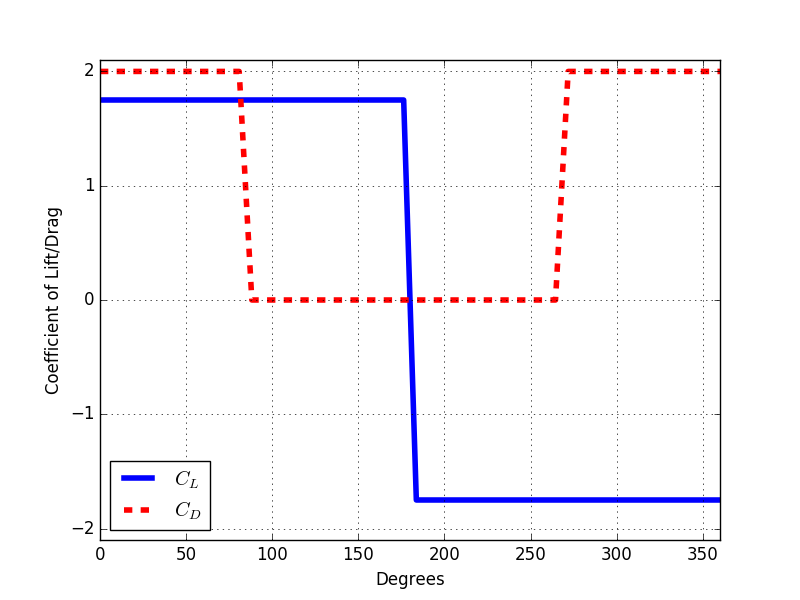
\includegraphics[width = 12 cm]{figs/opt_drags}
    \caption{The idealized drag polars.} 
    \label{drags}
  \end{center}
\end{figure}

Under this approach, the steady state power extracted by the
turbine nearly doubled from the previous best attained with the 90
degree semicircles, to 2.1 kW.\todo{add info of energy extracted}

mention that flow would die if you didnt calibrate it


 The results of this model demonstrate a limit on how much of the energy
 can be extracted before disrupting the flow so greatly
 that the vortex cannot be maintained.

add images of the optimal runs\todo{add opt drag polar images}